% Schematic of one A100 SM (slides 8-9)
\begin{figure}[ht]
\centering
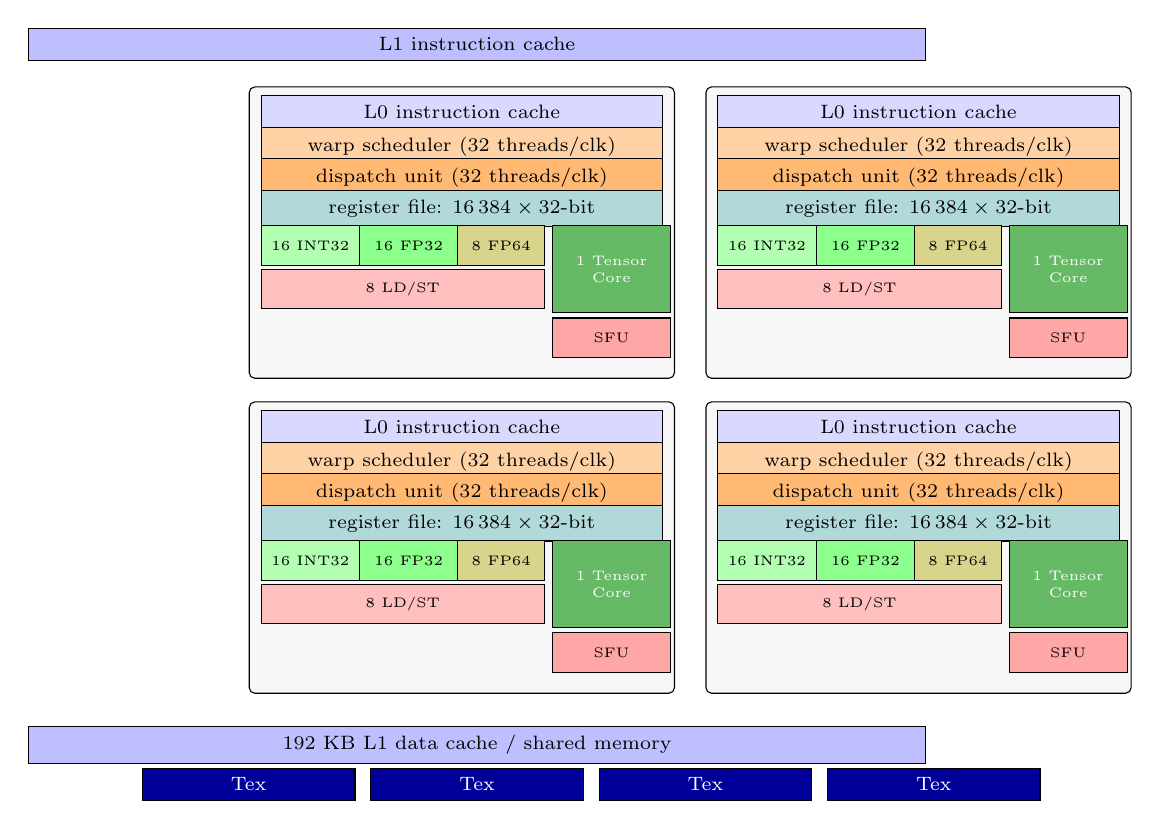
\begin{tikzpicture}[font=\scriptsize,
  part/.style={draw,rounded corners=2pt,fill=gray!6,minimum width=5.4cm,minimum height=3.7cm},
  bar/.style={draw,minimum width=5.1cm,minimum height=0.36cm,align=center},
  unit/.style={draw,minimum height=0.5cm,align=center}]
  \node[bar,fill=blue!25,minimum width=11.4cm] at (2.9,8.45) {L1 instruction cache};
  \foreach \px/\py in {0/4.2, 5.8/4.2, 0/0.2, 5.8/0.2}{
    \begin{scope}[shift={(\px,\py)}]
      \node[part,anchor=south west] at (0,0) {};
      \node[bar,fill=blue!15,anchor=north west] at (0.15,3.6) {L0 instruction cache};
      \node[bar,fill=orange!35,anchor=north west] at (0.15,3.2) {warp scheduler (32 threads/clk)};
      \node[bar,fill=orange!55,anchor=north west] at (0.15,2.8) {dispatch unit (32 threads/clk)};
      \node[bar,fill=teal!30,anchor=north west] at (0.15,2.4) {register file: $16\,384\times32$-bit};
      \node[unit,fill=green!30,minimum width=1.25cm,anchor=north west,font=\tiny] at (0.15,1.95) {16 INT32};
      \node[unit,fill=green!45,minimum width=1.25cm,anchor=north west,font=\tiny] at (1.4,1.95) {16 FP32};
      \node[unit,fill=olive!35,minimum width=1.1cm,anchor=north west,font=\tiny] at (2.65,1.95) {8 FP64};
      \node[unit,fill=green!55!black!60,minimum width=1.5cm,minimum height=1.1cm,anchor=north west,text=white,font=\tiny] at (3.85,1.95) {1 Tensor\\Core};
      \node[unit,fill=red!25,minimum width=3.6cm,anchor=north west,font=\tiny] at (0.15,1.4) {8 LD/ST};
      \node[unit,fill=red!35,minimum width=1.5cm,anchor=north west,font=\tiny] at (3.85,0.78) {SFU};
    \end{scope}
  }
  \node[bar,fill=blue!25,minimum width=11.4cm] at (2.9,-0.45) {192 KB L1 data cache / shared memory};
  \foreach \i in {0,1,2,3}{\node[bar,fill=blue!60!black,text=white,minimum width=2.7cm] at (0.0+2.9*\i-0.0,-0.95) {Tex};}
\end{tikzpicture}
\caption{One A100 SM drawn as four identical sub-partitions that share the L1/shared-memory block and the
texture units (compare slide~8). Multiplying the per-partition numbers by four gives $64$ FP32, $64$ INT32,
$32$ FP64 units, $4$ Tensor Cores and a $65\,536$-entry register file for the whole SM.}
\label{fig:sm}
\end{figure}
